\subsection{Timing}

Electrical signals propagate at a finite speed. Because of this, electrical components used to implement logic gates have a non-zero propagation time, after which the manufacturer guarantees that the output signal has settled at the expected voltage level. Since many of these individual logic gates are connected in series, their propagation delays add up, as do the propagation times of the traces between the circuits. The propagation times of logic gate \acp{ic} are typically on the order of 10s of nanoseconds. The propagation speed of electromagnetic waves in any given material is given by \cite{heule2016stratified}

\begin{displaymath}
    v_s = \frac{c}{\epsilon_r}
\end{displaymath}

On a \ac{pcb} using the widely used material FR-4, which has a relative permittivity of $4.4$ \cite{azar1996experimental}, this comes to $\approx \SI[per-mode=symbol]{1.43}{\centi\metre\per\nano\second}$. Considering that the distances between \ac{ic} terminals are on the order of individual millimetres, this is negligible in most cases. Additionally, much of the distance a signal travels is between the terminals of an individual \ac{ic}, i.e internal to the \ac{ic}, which is already included in the propagation delay of that component.

When a logical expression is implemented as a tree of logic gate components, the propagation delays of each branch must be added, since the inputs of any given \ac{ic} must have settled before the propagation continues. For each such tree, there is a critical path. This is the branch with the highest total propagation delay. Since all other branches will have settled earlier than this branch, it dictates the required propagation delay of the entire expression. \autoref{fig:critical_path} shows the critical path of the expression $(A \land B) \land \lnot \lnot \lnot C$. Even though the lowermost path has more components compared to the upper one, it has a lower propagation delay due to the lower propagation delay of each individual NOT gate. Therefore, the path containing only the two AND gates is considered the critical path. The total propagation delay of the whole circuit is therefore \SI{40}{\nano\second}.

\begin{figure}[h!]
    \centering
    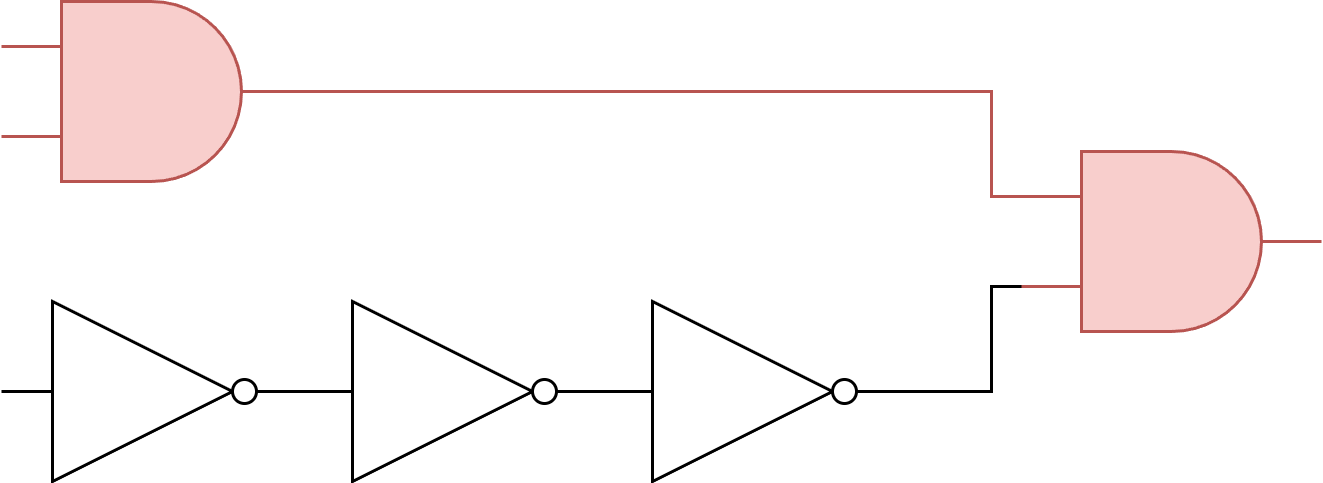
\includegraphics[width=0.7\textwidth]{images/drawio/critical_path.png}  % Replace with your image file
    \caption[Critical path]{Critical path shown in red, assuming a propagation delay of \SI{20}{\nano\second} per AND-Gate and \SI{5}{\nano\second} per NOT-Gate}
    \label{fig:critical_path}
\end{figure}

\paragraph*{Combinatorial and sequential logic} \label{sec:fundamentals_timing_sequential}

Combinatorial logic describes a circuit of digital gates that compute some pure boolean function. This means that the output of the circuit depends only on the present input and not on the history of the input. This contrasts with sequential logic, in which, as the name suggests, the output also depends on the order of operations, i.e an output may depend on previous inputs. In a digital electrical computer, this can be realised by forming loops between logic gates. An example of a combinatorial logic circuit is an adder circuit. There is no state stored within the circuit, it need not know the results of its previous operation to calculate any other addition. Once the input signals have been applied and propagated through the logic circuit, the system is stable. There are no feedback loops that may cause the circuit to change state at any point if the inputs remain stable. An example of a sequential logic circuit is the venerable SR latch. Such a latch can be seen in \autoref{fig:nand_sr_latch}.

\begin{figure}[h!]
    \centering
    \begin{minipage}{0.6\textwidth}
        \centering
        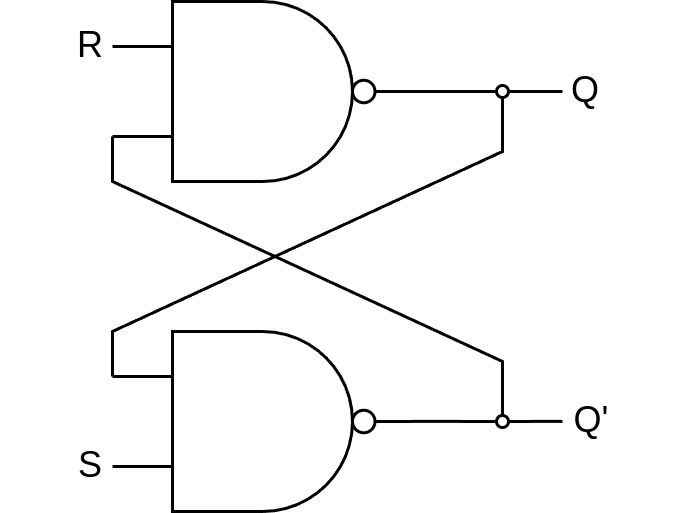
\includegraphics[width=0.7\textwidth]{images/drawio/nand_latch.png}  % Replace with your image file
        \caption{SR Latch made from NAND gates}
        \label{fig:nand_sr_latch}
    \end{minipage}
    \begin{minipage}{0.35\textwidth}
        \centering
        \vspace{-3em}
        \begin{align}
            Q' &= R \lnand Q \label{equ:latch_q_not} \\
            Q &= S \lnand Q' \label{equ:latch_q}   \\
            Q &= S \lnand (S \lnand Q') \nonumber  \\
            Q &= S \lnand (S \lnand (S \lnand Q')) \nonumber  \\
            Q &= \dots \nonumber 
        \end{align}
    \end{minipage}
\end{figure}

Within such a latch, there are clearly cycles, where the output of each NAND gate serves as the input of the other NAND gate. The boolean expressions for $Q$ and $Q'$ are given in equations \ref{equ:latch_q} and \ref{equ:latch_q_not}. Even though one can write an expression for each path through the latch, when expanding any one of the two, there is an unbounded recursion:

This is a problem when analytically analysing such circuits. However, in real hardware, due to inherent propagation delays, the system settles into one of two possible stable states; it is therefore called bistable. In practice, this latch circuit is used for storing the state of an individual bit. Due to tolerances in hardware manufacturing, it is not trivial to build perfectly timed combinatorial circuits, especially in mass manufactured goods such as \acp{ic}. For this reason, a combination of sequential and combinatorial circuits is used. Combinatorial circuits perform certain mathematical and logical operations, as they do not require any previous state, while sequential circuitry is used to retain state in components such as memories and registers. To synchronise the operation of all sequential circuits, a global clock signal is introduced. On each rising or falling edge of this signal, the state of certain or all state storage circuits is updated. Then, from this new state, the combinatorial circuits compute their new outputs, which are then stored on the next rising or falling edge of the clock.

The clock signal is an approximation of a square wave in most designs. Because only the time information is interesting, it is important to make the timing information as precise as possible. Due to the manufacturing tolerances of the components which are used to detect rising or falling edges, steeper clock signal edges are preferrable. When both falling and rising edges of a clock signal are used for instructing circuits with different propagation delays, the width of the HIGH and LOW signal phase may be asymmetrical to reflect this. This approach avoids unnecessary downtime but requires more complex signal generation logic.